<<<<<<< HEAD
\section{Implementation}

\subsection{SketchImporter}

This component is implemented as a \textit{Tool} and is an extension of \textit{ImageTool}. But only the \textit{creationFinished} method is overwritten. The \textit{ImageTool} already provides a functionality to import an image to the drawing. With the extension this image is set to the background and positioned to the (0,0) point. As the \textit{ImageTool}, this component also requires an \textit{ImageFigure} as constructor parameter and interact directly to the current view of this JHotDraw application.

For the implementation of the SketchImporter component two classes were created: The \textit{BackgroundImageTool} and the \textit{ZeroPointMoveAction}. The second one is just a helper class which is used by the other to move the imported image to the "`zero point"' (0,0) and therefore extends the abstract \textit{MoveAction}.
The \textit{BackgroundImageTool} extends the \textit{ImageTool}-class provided by JHotDraw. The basic image import is already implemented there. The imported image is only moved to the right location and set as background. Therefore the \textit{DrawingView} has to be used, which could be accessed through the \textit{getView} method.

\begin{figure}[h]
    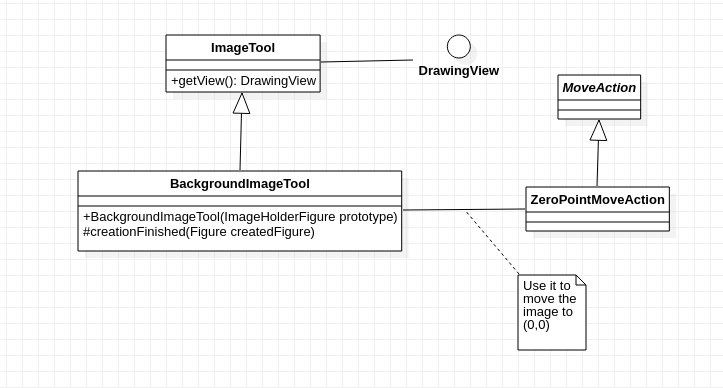
\includegraphics[keepaspectratio,width=\textwidth]{images/SketchImporter.png}
    \caption{SketchImporter Implementation}
\end{figure}

\subsection{Walls, Doors, Windows}

Wall, Door and Window are extending ImageFigure.
Also, Door and Window are created by a special CreationTool named "CreateInWallElement".
It checks that doors and windows are always placed on a wall.
If not, it intercepts the call of the framework to mousePressed.
